\chapter{Evaluation}
In questo capitolo verrà spiegata come è stata effettuata la valutazione delle perfomance del plug-in. Le perfomance sono state valutate in termini di \textbf{efficacia}, ovvero, quanto siano accurate le previsioni effettuate, ed \textbf{efficienza}, ovvero, quanto tempo, spazio e CPU utilizza il plug-in.   

\section{Metodologia utilizzata}
\label{sec:metodologiaevaluation}
L'analisi qualitativa e qualitativa è state effettuata cercando di calare quanto più possibile il plug-in in un contesto reale. Per fare cioè esso doveva effettuare le sue predizioni su degli input che non aveva mai visto. A tal fine è stato scelto da \href{https://www.kaggle.com/}{kaggle.com} il dataset {\tt Sentiment140 dataset with 1.6 million tweets }\cite{sentiment140} dalla quale sono state selezionate 500 entry con una funzione {\tt random}.

Per inviare le 500 entry al backend di Knoxly è stato realizzato un bot con \href{https://selenium-python.readthedocs.io/}{Selenium with Python}. Esso interagisce con una pagina web e inviava la frase al backend secondo i criteri definiti  dall'euristica per l'invio della frase(Sez. \ref{sec:frontend}).

Durante l'invio delle frasi il backend registra tempo(in secondo), RAM utilizzata e CPU utilizzata, mentre, il backend misura RAM e CPU utilizzata con e senza l'utilizzo di Knoxly.

Infine i risultati vengono raccolti e mostrati sotto forma di grafici e matrici.

\begin{figure}[h!t]
    \centering
    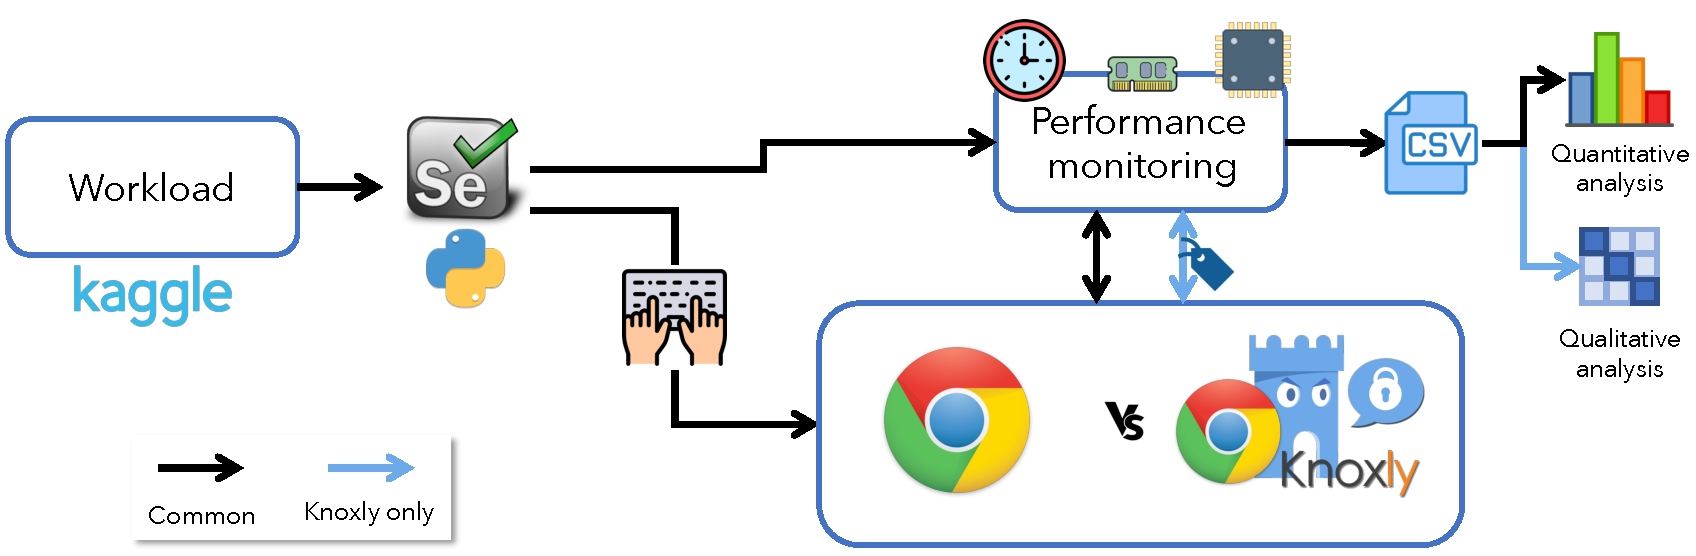
\includegraphics[width=15cm]{Figure/grafici/evaluation_cropped.pdf}
    \caption{Workflow della metodologia utilizzata}
    \label{fig:methodeval}
\end{figure}
\FloatBarrier

\section{Qualitative Analysis}
\label{sec:quantitative}
Una analisi qualitativa è stata effettuata al fine di valutare le performance sia del backend che del frontend in termini tempi di esecuzione, \%CPU utilizzata e RAM utilizzata.
\subsection{Server-side}
\label{sec:quantbackend}
Delle frasi che sono state inviate al backend vengono prese le seguenti misure:
\begin{itemize}
    \item \textbf{Tempo}: per tempo si intende solo il tempo in secondi impiegato dal server per smaltire la richiesta che gli è arrivata. Questa misura non tiene conto della latenza fra client e server
    \item \textbf{\% Utilizzo CPU}: percentuale di CPU utilizzata dal server per smaltire una richiesta 
    \item \textbf{RAM allocata}: Mb di RAM utilizzati dal server per smaltire una richiesta
\end{itemize}

\paragraph{Tempo}

\begin{figure}[h!t]
    \centering
    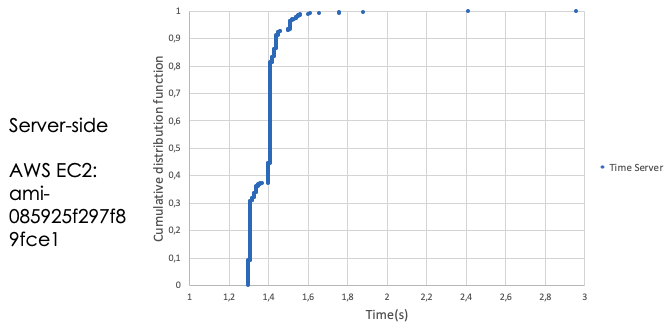
\includegraphics[width=15cm]{Figure/quantitativa/timeSrv.png}
    \caption{grafico dei secondi impiegati dal server per smaltire una richiesta}
    \label{fig:srvTime}
\end{figure}
\FloatBarrier

Si nota che il server in genere impiega dagli 1.3 agli 1.6 secondi per smaltire una richiesta, raramente impiega più di due secondi e che non impiega mai 3 secondi o più.

\paragraph{\% Utilizzo CPU}
\begin{figure}[h!t]
    \centering
    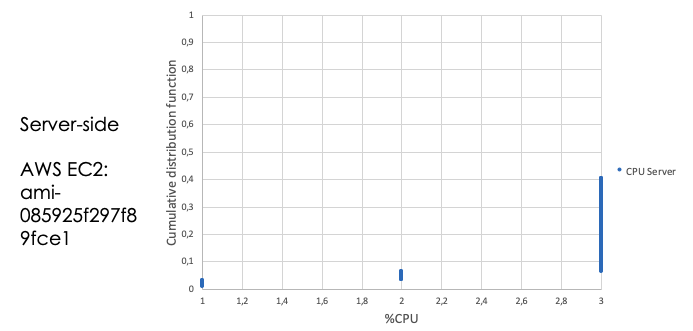
\includegraphics[width=15cm]{Figure/quantitativa/CPU-srv.png}
    \caption{grafico della percentuale di CPU impiegata per smaltire le richieste}
    \label{fig:srvCPU}
\end{figure}
\FloatBarrier

Si nota che il server generalmente utilizza il 3\% della sua CPU per smaltire le richieste  e che solo nelle fasi iniziali arriva ad utilizzare l'1 o il 2 percento della CPU.

\paragraph{RAM allocata}
\begin{figure}[h!t]
    \centering
    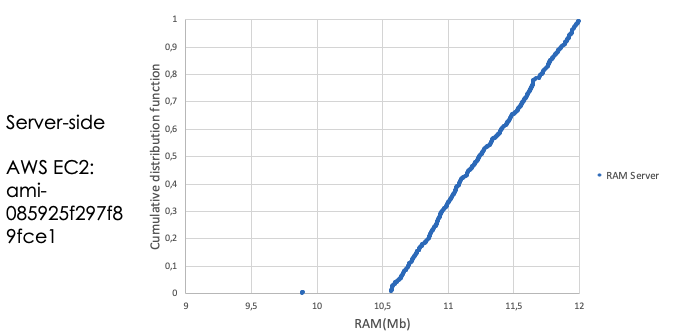
\includegraphics[width=15cm]{Figure/quantitativa/quant_RAM-srv.png}
    \caption{grafico dei Mb di RAM impiegati per smaltire le richieste}
    \label{fig:srvRAM}
\end{figure}
\FloatBarrier

Si nota che il consumo di RAM, lato backend, è compreso fra i 10.5 e i 12 Mb di RAM

\subsection{Client-side}
\label{sec:quantClient}
Delle frasi che sono state inviate al frontend vengono prese le seguenti misure:
\begin{itemize}
    \item \textbf{\% Utilizzo CPU Chrome e \%Utilizzo Knoxly}: percentuale di CPU utilizzata solo da Chrome durante l'invio delle frasi e percentuale di CPU utilizzata sola da Knoxly. 
    \item \textbf{RAM allocata da Chrome e RAM allocata da Knoxly}: Mb di RAM utilizzati da solo Chrome durante l'invio delle frasi e Mb di RAM utilizzati solo da Knoxly.
\end{itemize}

\paragraph{\% Utilizzo CPU Chrome e \%Utilizzo Knoxly}
\begin{figure}[h!t]
    \centering
    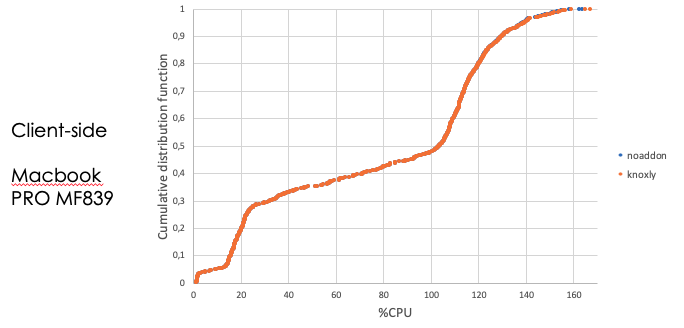
\includegraphics[width=15cm]{Figure/quantitativa/CPU-client.png}
    \caption{grafico della percentuale di CPU impiegata da Knoxly(punti arancioni) e da Chrome(punti blu)}
    \label{fig:clientCPU}
\end{figure}
\FloatBarrier

Dal grafico si evince che l'andamento dell'utilizzo delle percentuale di CPU solo di Knoxly è sovrapposto all'andamento dell'utilizzo della CPU solo da parte di Chrome. Quindi possiamo dire che Knoxly e Chrome utilizzano la stessa percentuale di RAM durante l'invio delle frasi e che Knoxly e Chrome al massimo arrivano ad utilizzare il 160\% della CPU,ovvero,poco più di un core e mezzo.

\paragraph{RAM allocata da Chrome e RAM allocata da Knoxly}
\begin{figure}[h!t]
    \centering
    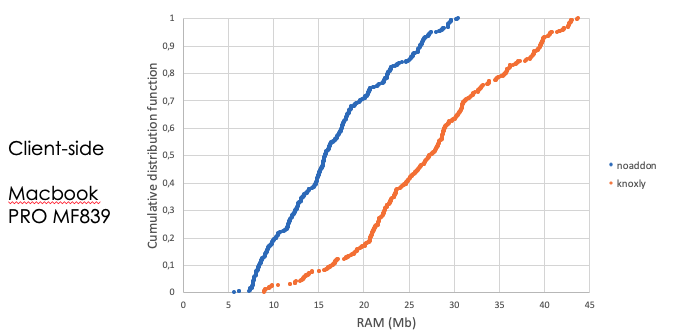
\includegraphics[width=15cm]{Figure/quantitativa/RAM-client.png}
    \caption{grafico dei Mb di RAM impiegati da Knoxly(punti arancioni) e da Chrome(punti blu)}
    \label{fig:clientRAM}
\end{figure}
\FloatBarrier
Dal grafico si evince che inizialmente Knoxly occupa più RAM rispetto a Chrome e questo può essere dovuto al fatto che il plug-in inizialmente deve caricare in memoria tutti i dizionari e le regexp di cui necessita per effettuare l'analisi lessicale e l'evidenziazione di un testo sensibile.



\section{Qualitative Analysis}
\label{sec:qualitative}
L'analisi qualitative è stata effettuata per valutare quanto i classificatori realizzati siano in grado di effettuare delle predizioni corrette. Per tenere traccia delle predizioni effettuate dai classificatori su un file {\tt csv} sono state salvate le frasi processate, il topic alla quale appartengono secondo la predizione effettuata dal {\tt Topic classifier} e la sensibilità della frase secondo la predizione effettuata dal {\\ Sensitiveness classifier}.

\subsection{Topic classifier}
\label{sec:qualTopic}

\begin{figure}[h!t]
    \centering
    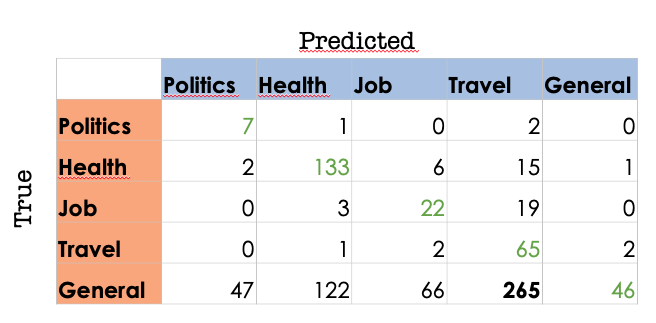
\includegraphics[width=15cm]{Figure/qualitativa/qual_topic.png}
    \caption{matrice di confusione del Topic classifier}
    \label{fig:confMtrTopicClass}
\end{figure}
\FloatBarrier

In Figura~\ref{fig:confMtrTopicClass} è mostrata la matrice di confusione ottenuta nella fase di evaluation. Si può notare che il Topic Classifier effettua il maggior numero di predizioni corrette sul topic health, mentre,il Topic classfier sbaglia spesso nel classificare una frase appartenente al topic general come una frase appartenente al topic travel. Questo a causa (a) del dataset utilizzato per l'addestramento che nel caso del topic \textit{travel} è fatto di tweet postati su Twitter (più simili morfo-sintatticamente a quelli utilizzati in questo test), nell'altro caso è una descrizione più articolata di una trama di un film (alquanto dissimile rispetto i testi utilizzati in questo test), (b) tweet molto brevi. Questo secondo problema è infatti motivo di molti errori.

Per questo motivo, abbiamo calcolato la media della lunghezza delle frasi contenute nel nostro workload ed abbiamo usato questo valore come soglia minima per considerare i tweet in una analisi che coinvolgesse solo quelle più lunghe. In particolare la media è 70 caratteri, per cui in questa seconda analisi consideriamo solo i tweet che contengono più di 70 caratteri.

\begin{figure}[h!t]
    \centering
    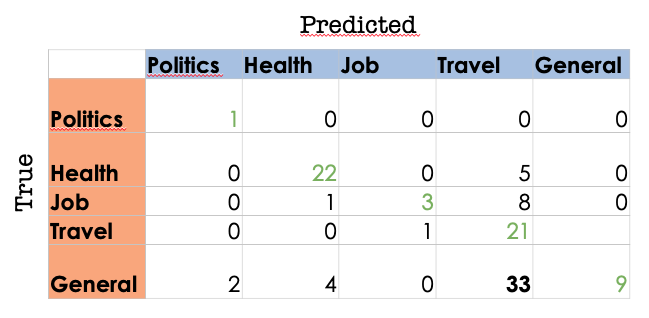
\includegraphics[width=15cm]{Figure/qualitativa/qual70char.png}
    \caption{matrice di confusione del Topic classifier dei soli testi maggiori di 70 caratteri}
    \label{fig:confMtrTopicClassGT70}
\end{figure}
\FloatBarrier

In Figura~\ref{fig:confMtrTopicClassGT70} è mostrata la matrice di confusione per il Topic classifier quando consideriamo solo tweet con lunghezza $l > 70$. L'ipotesi precedentemente formulata risulta vera. Infatti considerando solo frasi più lunghe il risultato migliora. Anche in questo caso si può notare che il topic con il numero più alto di veri positivi è health, seguito da travel. Il topic dove incontriamo maggiori errori di classificazione resta \textit{general}. Il Topic classifier anche su input più lunghi continua a sbagliare classificando come \textit{travel} frasi appartenenti a \textit{general}.

\subsection{Sensitiveness classifier}
\label{sec:qualSens}
Il secondo modulo di Knoxly di cui si vuole valutare l'efficacia è il Sensitiveness Classifier. Si osserva se una frase classificata come sensibile, quindi avendo con uno score di $probabilitaPositiva \geq 0.50$, è realmente sensibile in accordo alla euristica sulla sensibilità definita in Sez.~\ref{ssec:tblSens&Euricstic}. 

\begin{figure}[h!t]
    \centering
    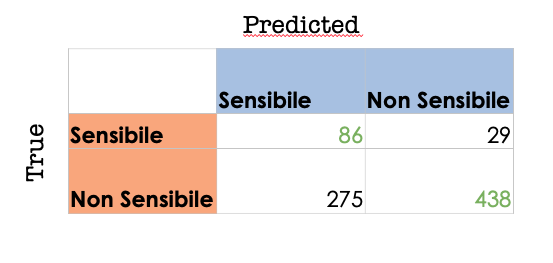
\includegraphics[width=15cm]{Figure/qualitativa/qualSens.png}
    \caption{matrice di confusione del sensitiveness classifier}
    \label{fig:sensitivenessevaluation}
\end{figure}
\FloatBarrier

In figura~\ref{fig:sensitivenessevaluation} è riportato il risultato di questa analisi di efficacia. Si può notare che il numero di falsi positivi è maggiore del numero dei falsi negativi. Da ciò si evince che il Sensitiveness Classifier individua e segnala più contenuti sensibili rispetto a quanti ne dovrebbe segnalare. Questo è un falso problema dal momento che si preferisce avere un classificatore che segnali un non sensibile come sensibile e non viceversa altrimenti dei dati sensibili e/o personali rischierebbero di essere divulgati in rete. Resta comunque il fatto che l'utente può addestrare il plug-in sul suo livello di privacy in base ai feedback che invia, facendo così diminuire il numero di segnalazioni.

\subsection{Customized Sensitiveness classifier}
\label{sec:qualCusto}
Per testare il modulo di Customized Sensitiveness Classifier abbiamo automatizzato con Selenium la digitazione di testo in linguaggio naturale e l'invio feedback al customized sensitiveness classifier lato client. L'idea è stata quella di preparare un dataset di testi che risultano essere sensibili e farli classificare al customized sensitiveness classifier. Per ciascun testo, vogliamo inviare a Knoxly un feedback negativo e ripetere la classificazione dell'intero dataset. Ci aspettiamo che se il customized sensitiveness classifier apprende in modo corretto dall'utente, allora l'accuratezza risultante dalla classificazione diminuisce con l'aumentare dei feedback.

Per questo esperimento abbiamo utilizzato un dataset minimale, composto da 10 elementi sensibili per ciascun topic (health, politics, travel, general, job). Abbiamo incrementato la taglia di questo dataset del 200\% popolandolo con frasi di significato simile ma scritte in altre lingue (italiano in particolare) o utilizzando sinonimi. Per il primo caso abbiamo utilizzato deepl\footnote{\url{https://www.deepl.com/translator}}, un famoso..., nel secondo invece, Reverso\footnote{\url{https://synonyms.reverso.net/synonym/}}, un servizio online che aiuta gli utenti nelle traduzioni domain-specific e nella ricerca di sinonimi. In tabella~\ref{tab:datasetcustomized} ne è riportato un esempio per il topic travel.


\begin{table}[h!t]
\centering
\begin{tabular}{l|p{9cm}}
\toprule
\textbf{Frase originale} & united Not sure what you are talking about She is going on nonstop flights SNA to SFO and then SFO to EWR \\
\midrule
\textit{Reverso} & united Not sure what you are speaking about She is riding on nonstop flights SNA to SFO and then SFO to EWR \\ 
\midrule
\textit{deepl} & united Non so di cosa stai parlando Lei sta andando su voli nonstop da SNA a SFO e poi SFO a EWR \\
\bottomrule
\end{tabular}
\label{tab:datasetcustomized}
\caption{Esempio di data-augmentation per il dataset Travel nell'esperimento di efficacia per il Customized Sensitiveness Classifier. \textit{Reverso}: refactoring della frase utilizzando il famoso servizio online, \textit{deepl}: traduzione della frase dall'inglese all'italiano.}
\end{table}
\FloatBarrier

Il risultato dell'esperimento è incoraggiante in quanto tutti i classificatori diminuiscono le loro performance via via che l'utente (bot selenium in questo caso) invia feedback negativi. In particolare in Figura~\ref{fig:plot_acc-health} e Figura~\ref{fig:plot_acc-travel} si mostrano i risultati ottenuti per Health e Travel, rispettivamente. Notiamo che, nel caso di Health, bastano pochi feedback per migliorare la conoscenza del classificatore e far adattare le sue segnalazioni alla percezione utente di privacy. Nel caso di Travel invece, l'utente ha bisogno di inviare più feedback prima che il classificatore comprenda le sue esigenze, in particolare ha bisogno di circa 10-12 feedback prima di apprendere bene "cosa si aspetta l'utente".

\begin{figure}[h!t]
    \centering
    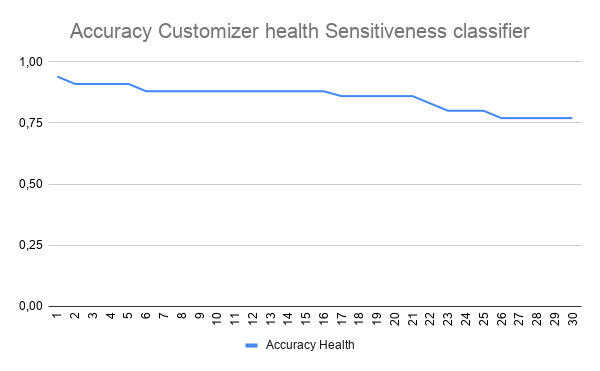
\includegraphics[width=15cm]{Figure/qualitativa/Custom_health-Sens.png}
    \caption{Scatter plot della accuracy del Customized Sensitiveness classifier sul topic health}
    \label{fig:plot_acc-health}
\end{figure}
\FloatBarrier

\begin{figure}[h!t]
    \centering
    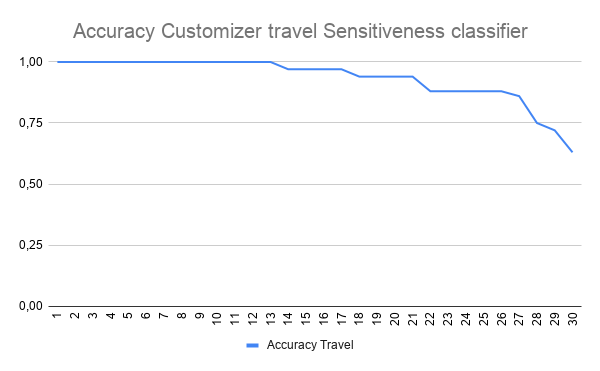
\includegraphics[width=15cm]{Figure/qualitativa/Customizer_travel-Sens.png}
    \caption{Scatter plot della accuracy del Customized Sensitiveness classifier sul topic travel}
    \label{fig:plot_acc-travel}
\end{figure}
\FloatBarrier

